% Created 2024-07-08 Mon 22:16
% Intended LaTeX compiler: pdflatex
\documentclass[11pt]{article}
\usepackage[utf8]{inputenc}
\usepackage[T1]{fontenc}
\usepackage{ragged2e}
\usepackage{caladea}
\usepackage{graphicx}
\usepackage{longtable}
\usepackage{wrapfig}
\usepackage{rotating}
\usepackage{epigraph}
\usepackage[normalem]{ulem}
\usepackage{hyperref}
\usepackage{amsmath}
\usepackage{amssymb}
\usepackage{capt-of}
\usepackage{hyperref}
\usepackage{fancyhdr}
\title{Novena à Santa Bibiana}
 % \hypersetup{
 %  pdfauthor={},
 %  pdftitle={Novena a/à SANTO_NOME},
 %  pdfkeywords={},
 %  pdfsubject={},
 %  pdfcreator={Emacs 29.4 (Org mode 9.6.15)}, 
 %  pdflang={English}
 % }

\title{
  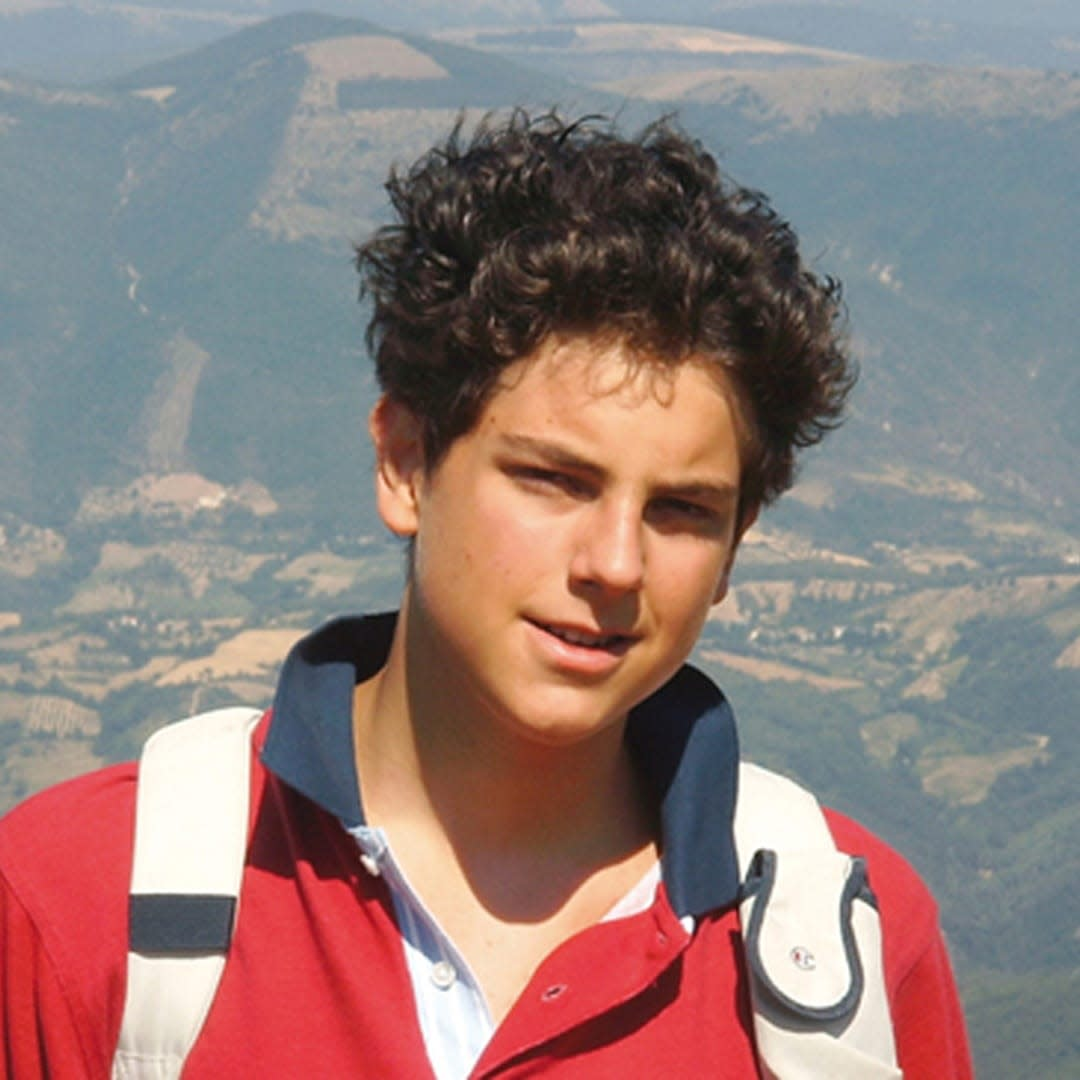
\includegraphics[scale=0.25]{./assets/imagem.jpg}
  \par
  NOVENA AO VENERÁVEL FULTON SHEEN}
\author{Garamog, Nina Freitas}
\date{30/11 - 08/12}
\renewcommand{\contentsname}{Sumário}

\begin{document}


\maketitle
\thispagestyle{empty}

\pagestyle{fancy}
\fancyhf{} % clear existing header/footer entries
\fancyfoot[LO, CE]{
  
\includegraphics[scale=0.2]{./assets/cross.png} Venerável Fulton Sheen, Rogai por Nós!
}
% Place Page X of Y on the right-hand
% side of the footer
\fancyfoot[R]{\thepage}
  
\newpage

\tableofcontents

\centering
\vfill
Visite-nos no Telegram: \url{https://t.me/CotidieNovena}
\newpage




%%%%%%%%%%%%%%%%%%%%%%%%%%%%%%%%%%%%% História  %%%%%%%%%%%%%%%%%%%%%%%%%%%%%%%%%%%%%%%%%%%
\section{História}\label{historia}

\begin{justify}


Fulton Sheen, arcebispo católico americano, destacou-se como bispo, comunicador e autor. Sua carismática presença na mídia nas décadas de 1950 e 1960 consagrou-o como um dos maiores comunicadores do século XX. Atraindo milhões de espectadores para os seus programas, sua capacidade única de se conectar ao público resultou em inúmeras conversões. O arcebispo não era apenas uma figura midiática, todos os dias ele passava uma hora inteira diante do sacrário nutrindo a sua fé e buscando a luz divina. Além disso, foi um grande intelectual, deixando uma vasta produção literária que combinava erudição teológica com uma comunicação envolvente. Atualmente reconhecido como Venerável Fulton Sheen, seu processo de beatificação está em andamento, fundamentado por suas virtudes heroicas reconhecidas e um milagre atribuído à sua intercessão.

\subsection{Os principais episódios da vida de Fulton Sheen}


\subsubsection{Nascimento e infância}

O seu nome de batismo era Peter John Sheen, mas gostava de ser chamado de Fulton Sheen — sendo Fulton o sobrenome de solteira de sua mãe. Ele veio ao mundo em 8 de maio de 1895, na cidade de El Paso, Illinois. Fulton Sheen foi o primogênito de Newton e Delia Sheen, que trabalhavam no campo e criaram-no com seus três irmãos em um ambiente de trabalho árduo e fé sólida.

Os pais de Fulton Sheen cultivavam uma grande devoção à Nossa Senhora, evidenciada pelo hábito diário de rezar o Rosário em família. Esse ambiente devoto levou-os a consagrar Peter ainda criança a Nossa Senhora, um ato solene que o bispo renovou no dia de sua primeira comunhão.

Desde cedo, Fulton Sheen demonstrou seu compromisso com a fé, sendo coroinha na catedral dedicada à Imaculada Conceição de Maria. Além disso, enquanto servia em uma missa celebrada pelo arcebispo local, um incidente envolvendo um objeto litúrgico tornou-se um momento profético. Após este acontecido, o arcebispo afirma que o jovem estudaria em Louvain e também se tornaria bispo um dia — fatos que realmente aconteceram posteriormente.

\subsubsection{Padre e intelectual}

Com uma aptidão precoce para a vida acadêmica, Fulton Sheen começou sua jornada sacerdotal ao ser ordenado padre aos 24 anos, em 20 de setembro de 1919, pelas mãos do Bispo Dunne. Desde cedo, sua promessa secreta a Deus de praticar diariamente a Hora Santa diante de Jesus Eucarístico e rezar a Missa de Nossa Senhora aos sábados destacou sua profunda devoção.

Após a ordenação, Sheen continuou seus estudos teológicos em Washington, na Universidade Católica da América. Ele se aprofundou em Direito Canônico e Sagrada Teologia, graduando-se nestas duas disciplinas. Embora mantivesse uma vida de estudos ativa, o sacerdote celebrava missa pela manhã e atendia paróquias nos feriados.

Além disso, movido por seu fascínio pelo neotomismo e o pensamento de Santo Tomás de Aquino, ele viajou para a Universidade de Louvain, na Bélgica, onde estudou também metafísica, psicologia e cosmologia. Em 1923, defendeu sua tese doutoral sobre “O Espírito da Filosofia Contemporânea e a finitude de Deus”, recebendo o Prêmio Cardeal Mercier — condecoração dada aos melhores trabalhos da instituição. Assim, com menos de 30 anos, Fulton Sheen já era doutor em filosofia.

\subsubsection{Bispo}

Ordenado bispo em Roma, em 1951, Sheen foi designado Bispo Titular de Cesariana pelo Papa Pio XII. Seus esforços missionários e sua influência na Igreja americana o marcaram como Bispo Auxiliar da Arquidiocese de Nova York. Além disso, de 1962 a 1965, ele participou ativamente das sessões do II Concílio do Vaticano.

\subsubsection{Bispo e estrela da TV}

Sheen se tornou uma figura notável ao iniciar o programa de rádio The Catholic Hour em 1930, alcançando milhões de ouvintes. No entanto, sua entrada triunfante na televisão ocorreu mais tarde, com os programas Life is Worth Living e The Fulton Sheen Program. Ao relacionar diversos temas com a fé católica, ele ofereceu respostas às questões existenciais, alcançando milhões de americanos e tornando-se uma voz relevante na sociedade da época.

Você sabia que Santa Clara é padroeira da televisão? Confira aqui.

\subsubsection{Exílio}

Após entrar em conflito com o Cardeal Spellman, Fulton Sheen foi designado para a pouco conhecida diocese de Rochester em 1966, quando tinha 71 anos. O cardeal, insatisfeito com a decisão do Papa Pio XII a favor de Sheen, jurou vingança, conseguindo encerrar o programa de TV de Fulton Sheen e forçar sua transferência. Ao enfrentar resistências e dificuldades com o próprio clero, Sheen renunciou em 1969, tornando-se bispo emérito de Rochester. Logo depois, o Papa Paulo VI o nomeou Arcebispo da Sé Titular de Newport (país de Gales), embora fosse uma diocese já extinta, apenas com título honorífico.

Desse modo, os últimos 13 anos da vida de Sheen foram de profunda purificação. Apesar de desafiador, esse período foi valioso para sua busca da santidade. Sua principal tentação sempre foi a vaidade e, mesmo como bispo, ele ainda lutava contra essa inclinação. E nestes anos finais, além de perder seu programa de televisão, Fulton Sheen permaneceu sem uma diocese para atuar, dedicando-se à escrita e à pregação.

\subsubsection{A morte de Fulton Sheen}

A vida deste arcebispo chegou ao fim de maneira comovente. Na sua ordenação sacerdotal, ele fez a promessa de rezar a Hora Santa Eucarística diariamente, assim, todos os dias passava uma hora inteira diante de Jesus Sacramentado. Em 9 de dezembro de 1979, aos 84 anos, o arcebispo descansou definitivamente diante do sacrário, onde costumava passar momentos em adoração.

Fulton Sheen cumpriu assim sua promessa fielmente até o último dia de sua vida. Desse modo, seu corpo foi encontrado morto diante do Sacrário, no dia seguinte. Inicialmente, ele foi enterrado na diocese de Nova York, sendo transladado para a diocese de Peoria, Illinois, em 2019. Seu túmulo agora pode ser venerado na Cathedral of Saint Mary of the Immaculate Conception.

\subsection{Fulton Sheen: o maior comunicador do século XX}

Fulton Sheen, reverenciado como o maior comunicador do século XX, deixou sua marca na era pós-Segunda Guerra Mundial com programas de televisão que conquistaram uma audiência monumental. Seu trabalho também desempenhou um papel fundamental ao confrontar as ideologias antagônicas ao Catolicismo que ganharam espaço nas universidades e na mídia após a década de 50. O bispo falava de Marx, Freud, Nietzsche e tratava de questões existenciais.

Em 1951, lançou o Life is Worth Living, um dos programas católicos mais influentes do século, transmitido por seis anos. Depois, na década de 60, apresentou outro sucesso, The Fulton Sheen Program, que foi ao ar de 1961 a 1968.

Enquanto Bispo Auxiliar de Nova York, interrompeu sua transmissão semanal de rádio para assumir o Life is Worth Living. Alcançou uma audiência ao vivo de 30 milhões de espectadores em horário nobre. Competindo com astros como Frank Sinatra e Milton Berle, superou em audiência, conquistando inclusive o Emmy de personalidade mais vista da televisão.

Embora falasse de Deus e do catolicismo, o objetivo do bispo era atrair e converter os não católicos. Desse modo, a temática do programa em si não era católica. Mas Fulton Sheen abordava questões existenciais, conectando os temas à fé católica, a fim de transmitir uma mensagem de fé aos espectadores.

Na plataforma da Lumine, você tem acesso ao programa mais célebre deste apóstolo da TV. A série A vida vale a pena reúne dez episódios da série original apresentada pelo Venerável Fulton Sheen, abordando temas como Eucaristia, revolução sexual e comunismo, além de assuntos relacionados à religião e à vida do homem moderno.


\end{justify}

\subsection*{Créditos }
\href{https://bibliotecacatolica.com.br/blog/devocao/vida-de-fulton-sheen/}{Minha Biblioteca Católica}

\newpage


%%%%%%%%%%%%%%%%%%%%%%%%%%%%%%%%%%%%% Orações  %%%%%%%%%%%%%%%%%%%%%%%%%%%%%%%%%%%%%%%%%%%
\section{Orações}\label{oracoes}

\subsection{Primeiro Dia}

“Não sei como Deus julgará minha vida, mas confio que Ele me verá com misericórdia e compaixão. Só tenho certeza de que haverá três surpresas no Céu. Em primeiro lugar, verei algumas pessoas que nunca esperei ver. Em segundo lugar, haverá várias pessoas que esperava que estivessem, mas que não estarão. E – mesmo confiando na misericórdia de Deus – a maior surpresa de todas pode ser o fato de eu estar lá. Quando é realizado o registro de qualquer vida humana, há três pares de olhos que a veem sob uma luz diferente: 1. Como eu a vejo. 2. Como os outros a veem. 3. Como Deus a vê”.

(Fulton J. Sheen)


\subsubsection{Oração}

Senhor, ajudai-nos a nos concentrar em Vós, como fez Fulton Sheen, para que sejamos humildes quando olharmos para nós mesmos, para que os outros vejam a Vós quando nos olharem e para que possamos ver nossa vida como a vedes Vós.

\textbf{\nameref{oracao-canonizacao}}


\subsection{Segundo Dia}

“Protestantes, judeus e católicos têm Deus, moralidade e religião em comum. Em nome de Deus, faremos nós judeus, protestantes e católicos – duas coisas: 

1. Perceber que um ataque a um é um ataque a todos, já que somos todos um em Deus; não precisamos de tolerância, mas de caridade; não de indulgência, mas de amor. 

2. Começar a fazer algo em relação à religião, e o mínimo que podemos fazer é rezar nossas orações; implorar as bênçãos de Deus sobre o mundo e nosso país; agradecer a Ele por suas bênçãos; e ser iluminados na plenitude de sua verdade. Fala-se demais sobre religião, e não se age o suficiente.” (Fulton J. Sheen)

(Fulton J. Sheen)


\subsubsection{Oração}

Senhor, Fulton Sheen alcançou pessoas de todas as religiões. Ajudai-nos a nos concentrarmos no que temos em comum, em vez de em nossas diferenças.

\textbf{\nameref{oracao-canonizacao}}


\subsection{Terceiro Dia}
“Em toda amizade, os corações crescem e se entrelaçam, de modo que os dois corações parecem formar apenas um coração com apenas um pensamento em comum. É por isso que a separação é tão dolorosa; não se trata tanto de dois corações se separando, mas de um só sendo despedaçado.” (Fulton J. Sheen)

\subsubsection{Oração}
Senhor, ajudai-me a construir amizades espirituais em minha vida para que eu possa me tornar um com meus irmãos, assim como todos nós seremos um no Céu. Acima de tudo, ajudai-me a perceber que separar-me de Vós significa um coração vazio para mim.

\textbf{\nameref{oracao-canonizacao}}


\subsection{Quarto Dia}
“A grande tragédia da vida não é tanto o que os homens sofreram, mas o que eles perderam. E que tragédia maior existe do que perder a paz do pecado perdoado? Não há um homem vivo que, caso o queira, não possa desfrutar do alimento e da bebida espirituais que Deus serve a todos que pedem.” (Fulton J. Sheen)

\subsubsection{Oração}

Senhor, Fulton Sheen conduziu tantas pessoas à paz da alma, dando-lhes a conhecer o vosso perdão. Ajudai-nos a compartilhar vossa dádiva de paz com outras pessoas, dando-lhes a conhecer o vosso verdadeiro e amoroso perdão e apresentando-lhes a dádiva da confissão.

\textbf{\nameref{oracao-canonizacao}}


\subsection{Quinto Dia}
“Todo amor nesta terra envolve escolhas. Quando, por exemplo, um rapaz expressa seu amor por uma jovem e pede que ela se torne sua esposa, ele não está apenas fazendo uma declaração de amor; ele também está negando esse amor a qualquer outra pessoa. Naquele único ato pelo qual a escolhe, rejeita tudo o que não é ela. Não há outra maneira real de provar que amamos uma coisa a não ser escolhendo-a em preferência a outra coisa. Palavras e sinais de amor podem ser, e muitas vezes são expressões de egoísmo ou paixão; mas atos são provas de amor. Podemos provar que amamos nosso Senhor somente se o escolhermos em preferência a qualquer outra coisa.” (Fulton J. Sheen)
\subsubsection{Oração}

Senhor, Fulton Sheen vos amava acima de todas as coisas. Ajudai-nos a escolher colocar-vos em primeiro lugar em nossas vidas, a fim de que possamos aprender o que é o verdadeiro amor.

\textbf{\nameref{oracao-canonizacao}}

\subsection{Sexto Dia}

“Queimar a vela nas duas pontas por causa de Deus pode ser tolice para o mundo, mas é um proveitoso exercício cristão para uma luz muito melhor! Apenas uma coisa importa na vida: ser considerado digno da Luz do Mundo na hora de sua visitação. Não devemos ter nenhum temor indevido por nossa saúde se trabalhamos arduamente pelo Reino de Deus: o Senhor cuidará de nossa saúde se cuidarmos de sua causa. De qualquer forma, é melhor se consumir do que se enferrujar”. (Fulton J. Sheen)

\subsubsection{Oração}

Senhor, mesmo cansado e doente, Fulton Sheen trabalhou incessantemente pelo vosso Reino. Ajudai-nos a aprender a trabalhar incansavelmente para Vós por meio de seu exemplo. Ajudai-nos a saber que não há descanso até que descansemos em Vós.

\textbf{\nameref{oracao-canonizacao}}


\subsection{Sétimo Dia}

“Maria não é apenas mãe de nosso Senhor e Salvador, Jesus Cristo, mas também é nossa mãe. Isso não é por um título de cortesia, por ficção legal ou por uma mera figura de linguagem, mas pelo direito de nos ter concebido em sofrimento ao pé da cruz… Maria, por sacrifício e obediência, recuperou para nós o título de Mãe dos vivos. Que destino ter a Mãe de Deus como minha mãe e Jesus como meu irmão!” (Fulton J. Sheen)

\subsubsection{Oração}

Senhor, Fulton Sheen aprendeu a obediência na escola de Maria. Ele tinha um relacionamento tão bom com ela que sabia que, quando estivesse diante do tribunal de Cristo, Vós diríeis: “Ouvi minha Mãe falar de ti”. Ajudai-nos a conhecer melhor Maria, a fim de que possamos ter o discernimento de tão grande obediência, amor, fé e esperança.

\textbf{\nameref{oracao-canonizacao}}


\subsection{Oitavo Dia}

“Se seguíssemos para a saúde as mesmas regras que seguimos na religião, todos estaríamos acamados. Não basta falar sobre a necessidade da saúde; precisamos fazer algo prático a respeito – por exemplo, comer, fazer exercícios e descansar. O mesmo acontece com a religião. Devemos nos alimentar com as verdades de Deus, exercitar nossos músculos espirituais em oração, mortificar-nos das coisas que são prejudiciais à alma e ser tão escrupulosos em evitar o mal moral quanto somos em evitar o mal físico.”

\subsubsection{Oração}
Senhor, Fulton Sheen não pediu aos outros que se confessassem ou que visitassem o Senhor uma hora por dia sem fazer isso ele mesmo. Ele praticava o que pregava. Protegei-nos da hipocrisia e ajudai-nos a levar outras pessoas a Vós por meio de nossas ações.

\textbf{\nameref{oracao-canonizacao}}

\subsection{Nono Dia}
“Quanto melhor nos tornamos, menos conscientes estamos de nossa bondade. Se alguém afirmar ser um santo, está mais próximo de ser um demônio. Jean Jacques Rousseau acreditava que, de todos os homens, ele era o mais perfeito; mas tinha tantas rachaduras em sua alma que abandonou seus filhos após o nascimento. Quanto mais santos nos tornamos, menos conscientes estamos de sermos santos. Uma criança é meiga enquanto não sabe que é meiga. Assim que pensa que é, torna-se impudente. A verdadeira bondade é inconsciente”. (Fulton J. Sheen)

\subsubsection{Oração}
Senhor, Fulton Sheen sempre se considerou um servo indigno e nunca se considerou um santo. Ajudai-nos a ser humildes em nosso serviço e a perceber, como Fulton Sheen percebeu, que todas as boas obras vêm de Vós.

\textbf{\nameref{oracao-canonizacao}}

\subsection{Oração para a canonização do Venerável Fulton Sheen} \label{oracao-canonizacao}

Pai Celestial, fonte de toda santidade, Vós suscitais na Igreja, em todas as épocas, homens e mulheres que servem com dedicação e amor heroicos. Vós abençoastes a Igreja por meio da vida e do ministério de vosso fiel servo, o Arcebispo Fulton J. Sheen. Ele escreveu e falou muito bem a respeito de vosso Divino Filho, Jesus Cristo, e foi um verdadeiro instrumento do Espírito Santo para tocar o coração de inúmeras pessoas. Se estiver de acordo com a vossa vontade, pela honra e glória da Santíssima Trindade e pela salvação das almas, pedimos que façais com que a Igreja o proclame santo. Fazemos esta prece por

\textbf{Pai-Nosso, Avé-Maria e Glória.}

\subsection*{Créditos:}
\href{https://bibliotecacatolica.com.br/blog/novenas/novena-de-fulton-sheen/}{Minha Biblioteca Católica}


\end{document}
